\documentclass[11pt,a4paper]{article}
\usepackage[T1]{fontenc}
\usepackage{lmodern,microtype}
\usepackage[a4paper,left=25mm,right=25mm,top=22mm,bottom=23mm,footskip=12mm]{geometry}
\usepackage{amsmath,graphicx,booktabs,array}
\usepackage[font=small,labelfont=bf,labelsep=period,hypcap=false]{caption}
\usepackage[hidelinks]{hyperref}
\hypersetup{pdftitle={Back-pressure effects in a converging--diverging air nozzle},pdfsubject={Axisymmetric flow and normal-shock verification}}
\graphicspath{{figures/}}
\setlength{\parindent}{1.2em}
\setlength{\parskip}{2pt}
\setlength{\abovecaptionskip}{5pt}
\setlength{\belowcaptionskip}{2pt}
\setlength{\emergencystretch}{1.2em}
\newcommand{\figcap}[2]{\captionof{figure}{#1}\label{#2}}
\newcommand{\tabcap}[2]{\captionof{table}{#1}\label{#2}}
\newcommand{\sourcepath}[1]{\texttt{\detokenize{#1}}}
\begin{document}
\begin{center}
  {\LARGE\bfseries Back-pressure effects in a\\[3pt] converging--diverging air nozzle\par}
  \vspace{8pt}
  {\normalsize Karim\enspace El\enspace Zahran}
\end{center}
\begin{abstract}
Four outlet pressures were imposed on a fixed nozzle to examine choking and the formation of an internal shock. A finite-volume solution of the axisymmetric Euler equations was compared with quasi-one-dimensional gas dynamics. At an inlet total pressure of 100~kPa and a back pressure of 75~kPa, the numerical pressure rise occurred 143.75~mm downstream of the inlet. The analytical shock position was 143.61~mm. The 0.14~mm difference is smaller than the finest axial cell width of 0.78~mm. The largest discrepancy in throat Mach number occurred at the theoretical onset of choking, where the medium grid gave 0.972.
\end{abstract}

\section{Geometry and boundary conditions}
The nozzle has equal inlet and exit areas and a throat halfway along its length. With axial coordinate $x$ measured from the inlet, the bore radius is
\begin{equation}
  r(x)=r_t\sqrt{1+\cos^2(\pi x/L)},\qquad
  L=200~\mathrm{mm},\quad r_t=10~\mathrm{mm}.
  \label{eq:bore}
\end{equation}
The end diameters are 28.284~mm and the throat diameter is 20.000~mm, giving $A_e/A_t=2$. Revolving the profile produces the 3D bore. The 2~mm radial wall in Fig.~\ref{fig:geometry} makes the cutaway visible. The flow calculation uses only the air passage.

\begin{center}
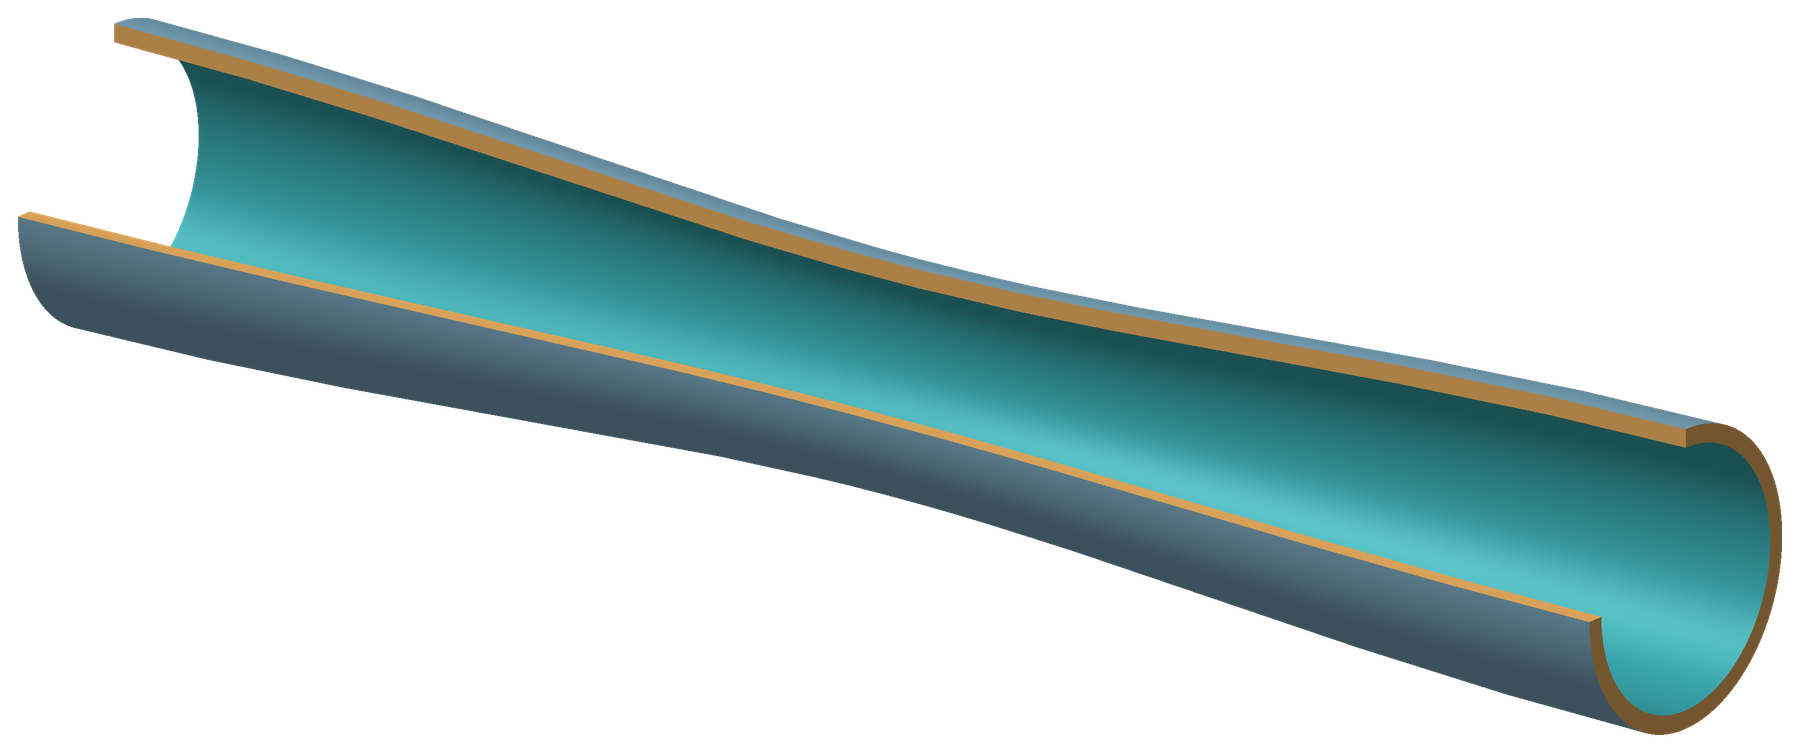
\includegraphics[width=.52\linewidth]{cad_cutaway.png}\\[1pt]
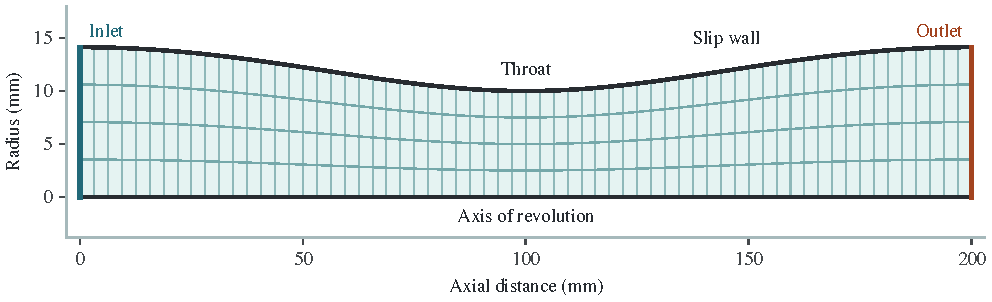
\includegraphics[width=.79\linewidth]{mesh.pdf}
\figcap{CAD cutaway (above) and meridional flow domain (below). The coarse mesh shows all 64 axial and four radial cells. The lower boundary is the axis of revolution.}{fig:geometry}
\end{center}
Air was treated as a calorically perfect gas with $\gamma=1.4$ and $R=287.05~\mathrm{J\,kg^{-1}\,K^{-1}}$. Inlet flow was axial, with total pressure $p_{01}=100$~kPa and total temperature $T_{01}=300$~K. The wall was adiabatic with slip. The specified back pressure $p_b$ set the exit static pressure for subsonic outflow. Once the exit became supersonic, the solver extrapolated the exit state from the interior. All pressures reported here are absolute.

\newpage
\section{Analytical reference and numerical method}
\subsection{Area change and shock fitting}
For steady isentropic flow, a section with $A>A^*$ admits a subsonic and a supersonic Mach-number solution. With $A^*$ denoting the sonic area associated with the local total pressure, the reference solution uses~\cite{ames}
\begin{equation}
 \frac{A}{A^*}=\frac{1}{M}
 \left[\frac{2}{\gamma+1}\left(1+\frac{\gamma-1}{2}M^2\right)\right]^{\frac{\gamma+1}{2(\gamma-1)}},
 \qquad
 \frac{p}{p_0}=\left(1+\frac{\gamma-1}{2}M^2\right)^{-\gamma/(\gamma-1)}.
 \label{eq:isentropic}
\end{equation}
At choking, $A^*=A_t$ upstream of any shock. For $A_e/A_t=2$, Eq.~\eqref{eq:isentropic} gives the subsonic exit root $M_e=0.3059$ at incipient choking and the supersonic root $M_e=2.1972$ for matched expansion.

For an internal shock, a trial position $x_s$ fixes the upstream Mach number $M_1$ from the supersonic branch. The Rankine--Hugoniot relations then determine the downstream state~\cite{ames},
\begin{equation}
 M_2^2=\frac{1+(\gamma-1)M_1^2/2}{\gamma M_1^2-(\gamma-1)/2},
 \qquad
 \frac{p_2}{p_1}=1+\frac{2\gamma}{\gamma+1}(M_1^2-1).
 \label{eq:shock}
\end{equation}
The downstream total pressure follows from $M_2$ and $p_2$. The subsonic branch is continued to the exit, and $x_s$ is varied until $p_e=p_b$. At $p_b=75$~kPa this gives $M_1=1.763$, $M_2=0.625$ and $x_s/L=0.71804$. Comparing a numerical nozzle solution with this type of analytical reference follows the approach used in the NPARC verification archive~\cite{cdv}.

\subsection{Axisymmetric finite-volume calculation}
A custom C++ solver advanced mass, axial momentum, radial momentum and total energy on body-fitted quadrilateral cells. Each face flux was weighted by its radius, and the radial momentum balance included the cylindrical pressure source. The solver used a two-wave Harten--Lax--van Leer (HLL) flux~\cite{riemann}, piecewise-linear reconstruction and two-stage Runge--Kutta local pseudo-time stepping. The smooth, wholly subsonic case used centered slopes. A slope limiter was used in the other cases.

Each run stopped when all four residuals fell below $2\times10^{-5}$. For each nondimensional conservation equation, the residual was the sum of the absolute integrated cell imbalances divided by the inlet mass flux. The shock case was initialized with a trial jump at $x/L=0.62$. Its final location followed from the computed pressure distribution.

\begin{center}
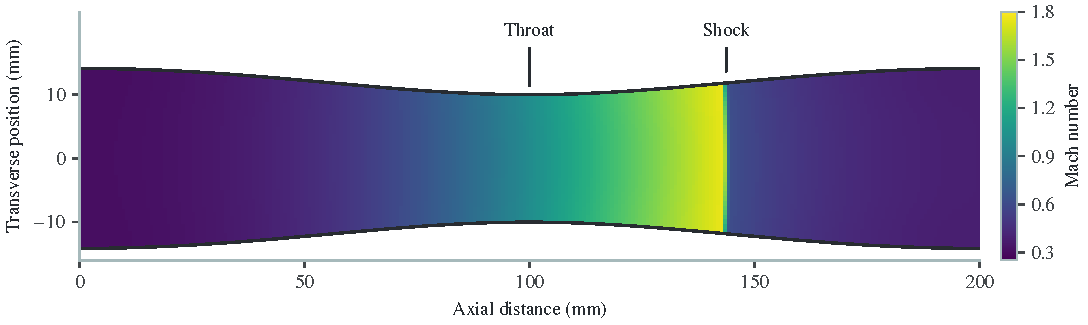
\includegraphics[width=.92\linewidth]{mach_field.pdf}
\figcap{Mach number at $p_b=75$~kPa on the $256\times16$ grid. The lower half mirrors the computed upper half. The transverse scale is enlarged.}{fig:field}
\end{center}

\newpage
\section{Effect of back pressure}
At $p_b=98$~kPa the throat Mach number was 0.361 and the divergent section recovered static pressure (Fig.~\ref{fig:sweep}). At the analytical choking limit, $p_b=93.716$~kPa, the calculated throat value rose to 0.972. The ideal solution reaches unity at a single axial station. The numerical value averages the adjacent cell-center results at this sharp maximum.

\begin{center}
\tabcap{Back-pressure sweep on the $128\times8$ grid. Throat and exit Mach numbers are cross-sectional area means. The CFD exit value is sampled in the last cell column.}{tab:cases}
\small\renewcommand{\arraystretch}{1.18}
\begin{tabular}{@{}lrrrrr@{}}
\toprule
 & $p_b$ & $M_t$ & $M_e$ & $M_e$ & $\dot m_{\rm in}$ \\
Flow condition & (kPa) & CFD & CFD & quasi-1D & (g/s) \\
\midrule
Subsonic                 & 98.000 & 0.3611 & 0.1701 & 0.1701 & 42.35 \\
Incipient choking\,$^a$   & 93.716 & 0.9717 & 0.3058 & 0.3059 & 73.27 \\
Internal shock           & 75.000 & 1.0001 & 0.3805 & 0.3803 & 73.31 \\
Matched supersonic exit  &  9.393 & 1.0001 & 2.1970 & 2.1972 & 73.31 \\
\bottomrule
\end{tabular}\\[4pt]
{\footnotesize $^a$Back pressure chosen from the analytical choking condition.}
\end{center}

\begin{center}
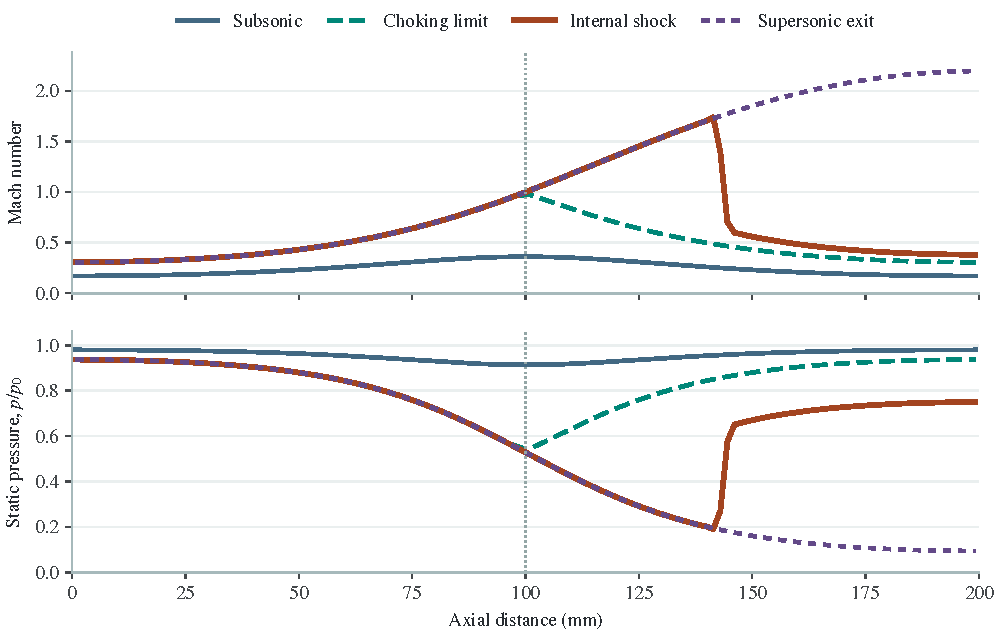
\includegraphics[width=.9\linewidth]{four_cases.pdf}
\figcap{Area-mean Mach number and static pressure along the nozzle for the four operating conditions in Table~\ref{tab:cases}. The dotted vertical line marks the throat.}{fig:sweep}
\end{center}

The 75~kPa and 9.393~kPa cases carried the same inlet mass flow to the precision shown. Their exit states differed substantially. At 75~kPa the air accelerated beyond Mach~1, passed through a shock and decelerated to $M_e=0.3805$. At 9.393~kPa the divergent section sustained supersonic flow to the exit. The overlapping upstream curves and the difference downstream show where back pressure affected these two choked solutions.

\newpage
\section{Shock location and grid sensitivity}
The numerical shock was assigned to the axial face across which the area-mean static pressure rose most sharply. Figure~\ref{fig:jump} shows the pressure rise and the corresponding Mach-number drop. The fine-grid transition spans several cells, whereas the analytical jump occurs at a single station.

\begin{center}
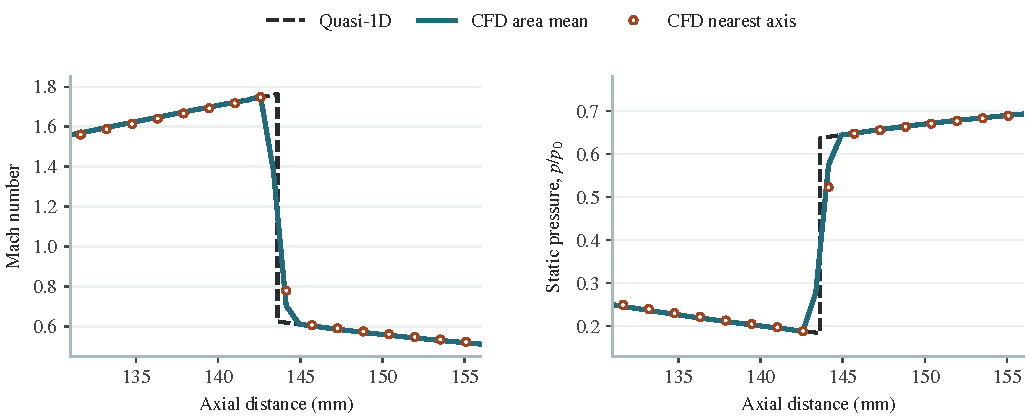
\includegraphics[width=\linewidth]{shock_detail.pdf}
\figcap{Fine-grid profiles through the shock at 75~kPa. Symbols sample the cells nearest the axis. The dashed curve is the independent quasi-one-dimensional solution.}{fig:jump}
\end{center}

\begin{center}
\tabcap{Mesh refinement at 75~kPa. Mass imbalance is $100\lvert\dot m_{\rm out}-\dot m_{\rm in}\rvert/\dot m_{\rm in}$. The analytical exit Mach number is 0.38034.}{tab:grids}
\small\renewcommand{\arraystretch}{1.16}
\begin{tabular*}{.93\linewidth}{@{\extracolsep{\fill}}lrrrr@{}}
\toprule
Grid & $\Delta x$ (mm) & $x_s$ (mm) & $M_e$ & Mass imbalance (\%) \\
\midrule
$64\times4$   & 3.125 & 143.75 & 0.38080 & $4.36\times10^{-4}$ \\
$128\times8$  & 1.563 & 143.75 & 0.38045 & $7.63\times10^{-6}$ \\
$256\times16$ & 0.781 & 143.75 & 0.38037 & $1.74\times10^{-6}$ \\
\bottomrule
\end{tabular*}
\end{center}

All three meshes contain a face at $x/L=0.71875$. Selecting that face on each grid limits what shock position alone can say about convergence. The exit Mach number provides a separate check. Its absolute difference from the analytical value fell from about $4.6\times10^{-4}$ on the coarse grid to $2.6\times10^{-5}$ on the fine grid.

\section{Conclusions}
For the 75~kPa case, the fine-grid shock location agreed with the analytical prediction to within one axial cell. At the onset of choking, the medium-grid throat Mach number remained 0.028 below the ideal value, despite close agreement at the exit. These comparisons test the inviscid internal-flow model. Prediction of wall friction, shock-induced separation or the external jet would require a different physical model and comparison with measurements.

\begingroup\small
\bibliographystyle{unsrt}
\bibliography{references}
\endgroup

\newpage
\appendix
\section{Convergence histories and project files}
Figure~\ref{fig:residual} shows the largest of the four equation residuals over the steady-state iterations for the internal-shock case. The coarse, medium and fine grids met the stopping criterion after 2,400, 5,700 and 14,700 iterations, respectively. Because each cell used a local pseudo-time step, the horizontal coordinate measures solver iterations.

\begin{center}
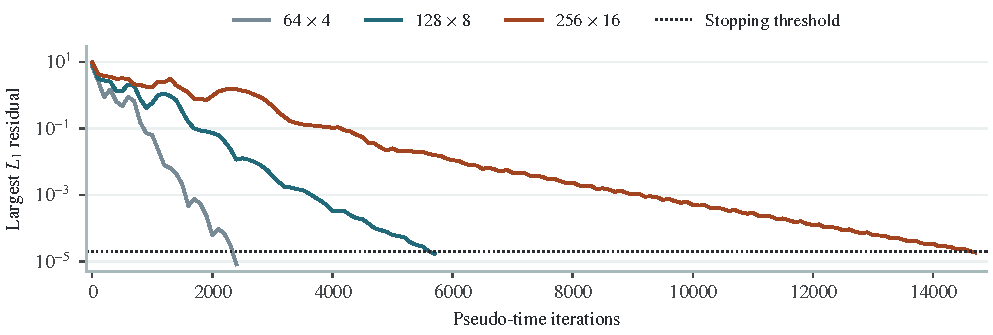
\includegraphics[width=.96\linewidth]{residuals.pdf}
\figcap{Convergence histories for the three grids at 75~kPa. The horizontal dotted line is the stopping criterion of $2\times10^{-5}$.}{fig:residual}
\end{center}
\subsection*{Geometry and flow fields}
The project archive contains separate STEP models for the hollow nozzle, the enclosed air volume and the meridional face used for meshing. The models were reimported into Open CASCADE for inspection. The recovered bore radius at the throat was 10.000~mm. The air volume was $94{,}247.78~\mathrm{mm}^3$, consistent with $\int_0^L \pi r^2(x)\,\mathrm{d}x=\tfrac32\pi r_t^2 L$.

\begin{center}
\small\renewcommand{\arraystretch}{1.25}
\begin{tabular}{@{}ll@{}}
\toprule
Quantity or operation & File in the complete CAD/CFD archive \\
\midrule
Three-dimensional nozzle & \sourcepath{CAD/Air_Nozzle_3D.step}\\
Meridional flow domain & \sourcepath{CAD/CFD_Fluid_Section_2D.step}\\
Fine-grid shock field & \sourcepath{Results/shock_256x16/flow.vtu}\\
All six run summaries & \sourcepath{Results/case_summary.csv}\\
Analytical profiles & \sourcepath{Results/quasi1D_reference.csv}\\
Reproduce the calculations & \sourcepath{Source/reproduce.py}\\
\bottomrule
\end{tabular}
\end{center}
The VTU files can be opened in ParaView. Each solution folder also includes axial profiles and the residual history in CSV format. The Fluent meshes and setup sheet support an independent calculation with the same boundary conditions. The numerical results reported here were generated with the C++ solver.
\end{document}
